\chapter{Codifica di canale}

\begin{figure}[h]
    \centering
    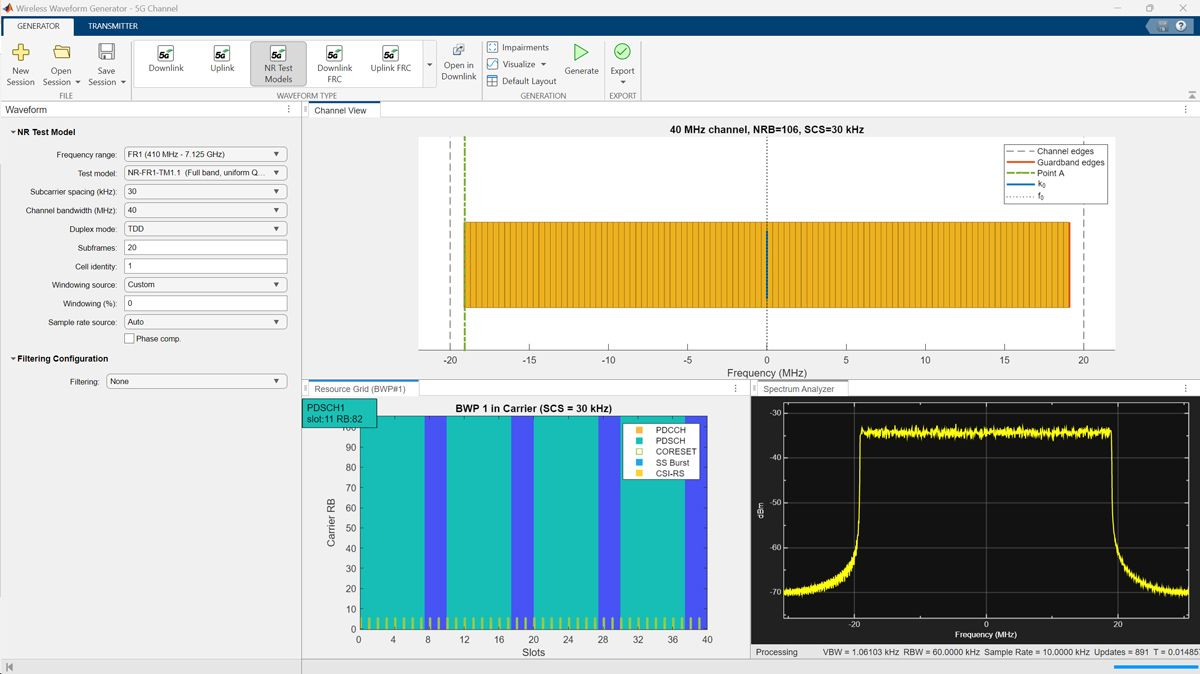
\includegraphics[scale = 0.35]{1718284029189.jpg}
\end{figure}

\newpage 

\section{Cosa è una codifica di canale}
\footnote{Slide del prof | Codifica di canale | pag 1 \\ 
Slide | Codifica di canale | pag  1\\
Appunti | 2025-04-14 | pag 7 - 8
} 

La codifica di canale è l'operazione mediane cui una trasmissione, in forma numerica, 
può essere protetta dagli effetti dei disturbi (soprattutto il rumore termico) introdotti dal canale e dagli apparati che elaborano il segnale. \newline 

Più precisamente, attraverso una opportuna strutturazione della sequenza dei simboli trasmessi, 
è possibile, in reazione, rivelare la presenza di errori o, meglio ancora, correggere fino a un numero prefissato, 
dipendente dalle caratteristiche del codice. \newline 

Si possono implementare diverse caratteristiche. \newline 

Faremo riferimento, per questo corso, il seguente schema più classico, definito "codifica a blocco": 

\begin{figure}[h]
    \centering
    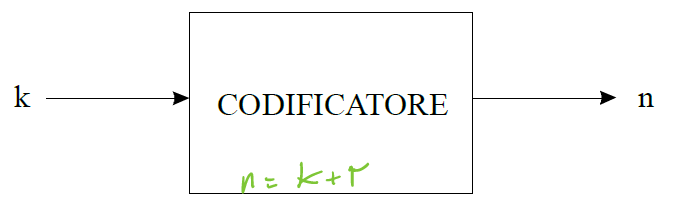
\includegraphics[scale = 1]{codifica a blocco.PNG}
\end{figure}

\begin{tcolorbox}
In questo corso, consideriamo solo gli errori dovuti al canale e non tratterremo su come è realizzato il codificatore e decodificatore.     
\end{tcolorbox}

Il codificatore opera su blocchi di k simboli in ingresso,
fornendone in uscita n, 
in cui: 

{
    \Large 
    \begin{equation}
        n > k 
    \end{equation}
}

Questo significa che, l'operazione di codifica introduce una certa ridondanza, 
cioè aggiungere r simboli, in particolare: 

{
    \Large 
    \begin{equation}
        r = n - k
    \end{equation}
}

che non portano informazione. \newline 

Benché l'operazione di codifica possa essere applicata tanto a canali binari quanto a canale M-ari, 
di seguito ci riferiremo esclusivamente al caso binario. \newline 

La possibilità di rivelare o correggere errori in una sequenza di simboli è legata alla capacità di individuare, 
in ricezione, sequenze che non potevano essere trasmesse. \newline 

Se la sorgente emette simboli binari (cioè bit) equiprobabili ed incorrelati, 
un blocco di k simboli può assumere qualunque delle $2^{k}$ sequenze possibili. \newline 

L'aggiunta degli r simboli di ridondanza, al contrario, consente di differenziare maggiormente le sequenze trasmissibili (alfabeto di trasmissione). \newline 

Avendo a disposizione n simboli, si possono infatti "sintetizzare" $2^{n}$ sequenze, 
ma essendo necessarie solo $2^{k}$ sequenze (cioè la parola di codice) 
la ridondanza potrà essere utilizzata proprio per differenziare maggiormente ciò che può essere trasmesso, 
riducendo il rischio di equivocazione. \newline 

\newpage 

\subsection{Codice a bit di parità}
\footnote{Slide del prof | Codifica di canale | pag 1 - 2\\ 
Slide | Codifica di canale | pag  1 - 2\\
Appunti | 2025-04-14 | pag 8
} 

Consideriamo l'esempio di "bit di parità": 
a partire da una sequenza di k di bit (con k arbitrariamente scelto) 
il codificatore aggiunge un altro simbolo binario, 
in modo che il numero totale di simboli "1" nella sequenza trasmessa sia pari. \newline 

Così facendo, 
solo metà delle $2^{n}$ sequenze vengono riconosciute come "ammissibili" in ricezione, 
dove: 

{
    \Large 
    \begin{equation}
        2^{n} = 2^{k+1}
    \end{equation}
} 

Se la sequenza ricevuta contiene un numero dispari di "1", 
il decodificatore riconosce che si è verificato almeno un errore. \newline 

Dunque, il sistema è in grado di ricevere la presenza di 1 errore senza peraltro essere in grado di correggerlo. \newline 

Ma, se il numero di errori è pari, il numero totale di simboli "1" torna ad essere accettabile. \newline 

Quindi, il decodificatore è inefficiente. \newline 

Visto in un'altra maniera, più elettronica e che viene implementata negli FPGA e negli LDPC, 
è che il codificatore del bit di parità è uno XOR di n ingressi, 
sia codificatore che al decodificatore. \newline 

\begin{tcolorbox}
    Se vuoi farti una cultura in merito: \newline 

    FPGA\\
    \url{https://www.ibm.com/it-it/think/topics/field-programmable-gate-arrays} \newline 

    LDPC\\
    \url{https://en.wikipedia.org/wiki/Low-density_parity-check_code} \newline 

    XOR \\
    \url{https://www.elemania.altervista.org/digitale/circuiti/circ2.html}

\end{tcolorbox}

Siccome con questo codice non si può rivelare l'errore, cioè capire dove c'è stato l'errore, 
o si può dire che è presente un errore o il ricevitore chiede al trasmettitore di inviare di nuovo la sequenza. \newline 

Oppure, si implementa un altro codice, come ad esempio il codice a ripetizione. \newline 

\newpage 

\subsection{Codice a ripetizione}
\footnote{Slide del prof | Codifica di canale | pag 2 \\ 
Slide | Codifica di canale | pag  2\\
Appunti | 2025-04-14 | pag 8 - 9
} 

Nel codice a ripetizione il valore k è prefissato e poniamo come esempio: 

{
    \Large 
    \begin{equation}
        k = 1
    \end{equation}
}

Nel codice a ripetizione, il codice replica n volte il simbolo emesso dalla sorgente. \newline 

Considerando un n uguale a: 

{
    \Large 
    \begin{equation}
        n = 5
    \end{equation}
}

il simbolo 0 generato dalla sorgente diventa: 

{
    \Large 
    \begin{equation}
        0 \to 00000
    \end{equation}
}

Continuando l'esempio, 
si supponga che, a seguito a degli errori trasmissione, 
la sequenza generata dal codice a ripetizioni diventa: 

{
    \Large 
    \begin{equation}
        00000 \to 10010
    \end{equation}
}

Il decodificatore riconoscerà che la sequenza ricevuta non potrà essere stata trasmessa. \newline 

Dovendo prendere una decisione sul simbolo inviato, 
il decodificatore riterrà più plausibile che sia stato trasmesso il simbolo 0 piuttosto che il simbolo 1. \newline 

Con questo criterio, il decodificatore sceglie "a maggioranza". \newline 

In questo esempio citato, il decodificatore sarà in grado di correggere fino a 2 errori. \newline 

Per una sequenza lunga n, è più probabile che avvenga un errore in un bit che in più bit. \newline 

In generale, per un codice a ripetizione di lunghezza n, il numero di errori correggibili è pari a: 

{
    \Large 
    \begin{equation}
        t = \left[ \frac{n - 1}{2} \right]
    \end{equation}
}

dove con le parentesi quadre di $\frac{n - 1}{2}$ si indica la parte intera di quel rapporto. \newline 

Ai fini delle capacità di correzione, non si ha alcun vantaggio ad assumere un n pari. \newline 

Portando un esempio con n = 6, si possono correggere 2 errori, 
che è lo stesso numero di errori che si possono correggere con n = 5. \newline 

Quindi, in generale, meglio utilizzare un numero n più basso possibile per correggere gli errori. \newline 

\newpage 

\section{Caratteristiche di una codifica di canale}
\footnote{Slide del prof | Codifica di canale | pag 2 \\
Slide | Codifica di canale | pag  2\\ 
Appunti | 2025-04-14 | pag 9 \\
Appunti | 2025-04-15 | pag 2 - 4
} 

Gli esempi descritti del codice a ripetizione e del codice a bit di parità, 
mettono in evidenzia due aspetti fondamentali e di validità generale: 

\begin{itemize}
    \item indipendentemente dal modo con cui viene implementata la decodifica, la stima in ricezione della sequenza trasmessa è generalmente basata su un criterio di massima verosimiglianza, chiamato anche criterio della minima distanza. \newline 
     Il decodificatore sceglie la parola di codice $\overrightarrow{v}$ più vicina dalla sequenza ricevuta $\overrightarrow{r}$ 
     \item la capacità di correzione è tanto maggiore quanto più le parole di codice sono diverse tra loro
\end{itemize}

\begin{tcolorbox}
In questa sequenza, codice e codifica verranno utilizzati come sinonimi. \newline 

Inoltre, per bit si intende sequenza di zeri e uni, e non si considerano bit informativi (si specificherà quando lo sono). 
\end{tcolorbox}

L'abilità di chi progetta il codice sta nell'individuare, 
a parità di altre condizioni, la parola di codice che meglio soddisfa la seconda proprietà. \newline 

Vi è un modo esplicito per quantificare la diversità tra le due sequenze di n simboli, 
che consiste nel misurare la relativa "distanza". \newline 

\begin{tcolorbox}
    Praticamente stiamo ritornando al concetto fatto sugli M vettori con N vettori di base fatto nelle varie modulazioni numeriche. \newline 

    Soltanto che, in questo caso, viene applicato questo concetto ad una sequenza di bit e non a dei vettori N-dimensionali. 
\end{tcolorbox}

\newpage 

\subsection{Distanza di Hamming}
\footnote{Slide del prof | Codifica di canale | pag 2 -3 \\ 
Slide | Codifica di canale | pag  2 - 3\\ 
Appunti | 2025-04-15 | pag 4 - 6
} 

Esistono vari tipi di definizioni di distanza: per adesso ci soffermiamo sulla definizione di distanza come distanza di Hamming. \newline 

La distanza di Hamming $d_{ij}$ tra due parole di codice $\overrightarrow{v_i}$ e $\overrightarrow{v_j}$ 
rappresenta il numero di posizioni per cui le due parole differiscono. \newline 

Ad esempio: 

{
    \Large 
    \begin{equation}
        \begin{cases}
        \overrightarrow{v} = 0001011
        \\
        \overrightarrow{j} = 0010110
    \end{cases}
    \to 
    d_{ji} = 4
    \end{equation}
} 

Le due parole di un codice a ripetizione di lunghezza n hanno distanza di Hamming n; e così via. \newline 

Dato un codice, si può definire la distanza minima, o semplicemente distanza di Hamming, tra due o più sequenze. \newline 

Per un codice generico, si dimostra che il numero di errori correggibili t è legato a $d_{min}$ dalle seguenti espressioni: 

{
    \Large 
    \begin{equation}
        d_{min}
        = 
        \begin{cases}
            2 \cdot + 1 \text{ se $d_{min}$ è dispari}
            \\
            2 \cdot + 2 \text{ se $d_{min}$ è pari}
        \end{cases}
    \end{equation}
}

Come si vede dalla formula di $d_{min}$, non comprare il numero n. \newline 

Questo significa che, all'aumentare di n, non è detto che si può correggere le sequenze. \newline 

\begin{tcolorbox}
    Un esempio concreto è quello che accade ogni giorno nell'ambito delle telecomunicazioni wireless: 
    la banda è stretta, quindi è sempre meglio inviare meno n bit possibili e quindi una $d_{min}$ minima per risolvere gli errori. 
\end{tcolorbox}

Il codice a bit di parità risulta un caso particolare di $d_{min}$ perchè la capacità di rivelazione degli errori è data da $d_{min} - 1$. \newline 

\newpage 

\subsection{Sottospazio di una decodifica}
\footnote{Slide del prof | Codifica di canale | pag 3 \\
Slide | Codifica di canale | pag  3\\  
Appunti | 2025-04-15 | pag 4 - 6 \\
Appunti | 2025-07-21 Ricevimento | pag 11 - 12.1
} 

Quando si genera un codice, dal punto di vista matematico, 
si genera un sottospazio rispetto a tutte le possibili configurazioni del bit. \newline 

I codici hanno diverse proprietà, di seguito ne elenchiamo due. \newline  

Se il codice è lineare, 
qualunque coppia di codice è presente solo la $d_{min}$. \newline 

\begin{tcolorbox}
    Per maggiori informazioni riguardo ai codici lineari: \newline 

    \url{https://en.wikipedia.org/wiki/Linear_code}
\end{tcolorbox}

Se il codice è sistematico, 
possono essere progettati con: 

{
    \Large 
    \begin{equation}
        n = d_{min}
    \end{equation}
}

fissa. \newline 

Ad esempio, il codice di Hamming può essere implementato con $d_{min} = 3$. \newline 

Se $d_{min}$ è bassa, può essere valutata e non stimata. \newline 

\begin{tcolorbox}
Per le codifiche "vecchie" si poteva valutare, quindi quantificare la distanza minima tra un simbolo rispetto all'altro perchè i simboli erano pochi. \newline 

Con le codifiche attuali, ciò non è possibile farlo perchè i simboli sono tanti e si utilizzano delle tecniche di codifica molto complicate: 
in questo caso, si dice che si può stimare la distanza minima, e non quantificarla come nelle codifiche "vecchie"
\end{tcolorbox}

Il codice opera quando il numero di errori non eccede le capacità correttive. \newline 

Cosa succede quando il numero di errori è maggiore di t? \newline 

Più frequentemente, nel tentativo di correggere la sequenza ricevuta, 
il decodificatore potrebbe aggiungere altri errori, 
con ciò "peggiorando" la situazione. \newline 

Consideriamo il seguente esempio: 

\begin{figure}[h]
    \centering
    \includegraphics[scale = 0.8]{Capacità correttiva di un codice esempio con n = 1.PNG}
\end{figure}

A rigore i vari sottospazi dovrebbero essere di dimensione n, 
ma nell'esempio in figura n = 1, quindi è un serie di punti lungo un segmento. \newline 

Le parole di codice sono contrassegnate dai cerchietti e separate da sequenze (contrassegnate con rettangoli) 
che possono essere ricevute, 
ma non corrispondono a parole di codice. \newline 

In figura, le due parole di codice $\overrightarrow{v_i}$ e $\overrightarrow{v_j}$ sono a distanza 5. \newline 

Ciascuna circonferenza, centrata su $\overrightarrow{v_i}$ e $\overrightarrow{v_j}$ ha raggio t, 
in cui t sono il numero di errori correggibili. \newline 

Se trasmessa la parola $\overrightarrow{v_i}$ e si riceve la sequenza $\overrightarrow{a}$ (in ricezione 3 simboli sono errati), 
il decodificatore stimerà, grazie al principio della vero-somiglianza (o anche chiamato della minima distanza), 
che la parola di codice più plausibile non è quella trasmessa che sia $\overrightarrow{v_i}$, 
bensì stimerà che la parola di codice trasmetta sia $\overrightarrow{v_j}$. \newline 

Ciò introduce 2 errori, pari alla distanza tra $\overrightarrow{a}$ e $\overrightarrow{v_j}$. \newline 

Per l'esempio preso in figura:

{
    \Large 
    \begin{equation}
        t = 2
    \end{equation}
}

cioè, al numero massimo di errori certamente correggibili. \newline 

Nel caso più sfortunato, il decodificato introduce, nel tentativo di correggere una situazione che eccede le sue capacità correttive, 
un numero uguale a t di errori addizionali. \newline 

\begin{tcolorbox}
Questo perchè, ritornando all'esempio, se io mando $\overrightarrow{v_i}$, 
ma ricevo $\overrightarrow{a}$ = $\overrightarrow{v_j}$, 
in quel caso il codice non può risolvere l'errore. 
\end{tcolorbox}

\newpage 

\section{Probabilità di un decodificatore di correggere un errore}
\footnote{Slide del prof | Codifica di canale | pag 3 - 5\\ 
Slide | Codifica di canale | pag  3 - 5\\ 
Appunti | 2025-04-15 | pag 6 - 7 \\
Appunti | 2025-07-21 Ricevimento | pag 12.2
}

Prima di implementare la codifica di canale, 
bisogna valutare l'efficienza del codice. \newline 

Tenendo conto anche delle osservazioni, 
si può concludere che la probabilità di decodificare correttamente una parola di codice soddisfa la seguente relazione: 

{
    \Large 
    \begin{equation}
        P_{rc}
        \ge
        \sum_{i = 0}^{t} 
        \binom{n}{i} \cdot p^{i} \cdot (1 - p)^{n-i}
    \end{equation}
}


dove p è la probabilità di transizione errata del singolo bit binario (da 0 a 1 o viceversa, 
in accordo con la definizione di canale binario simmetrico o BSC in inglese). \newline 

\begin{tcolorbox}
    Ricordiamo al volo come è fatto un canale BSC (che già avevamo introdotto nei capitolo precedenti). \newline 

    Il canale BSC causa questo cambiamento: \newline

    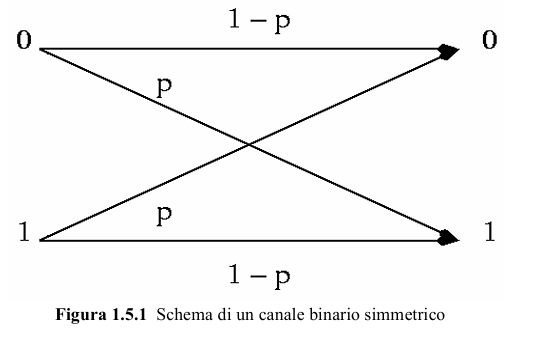
\includegraphics[scale = 0.8]{Schema canale BSC.PNG}

    cioè, se si trasmette uno 0, alla fine del canale, o può rimanere 0 o cambiare e diventare 1; 
    stessa cosa vale se è stato trasmesso un 1. \newline 

    La formula che esprime $P_{rc}$ è l'applicazione dell'esperimento di Bernoulli. \newline 

    Ti consiglio di ripassarlo dagli appunti del precedente corso. \newline 

    \url{https://github.com/ciccio25/appunti-teoria-dei-segnali/blob/main/Appunti%20Teoria%20dei%20segnali.pdf} \\
    Capitolo 12.6 - Esperimento di Bernoulli - pag 120 \newline 

    L'applicazione di Bernoulli lo possiamo applicare perchè alla fine il bit se è 0 o 1, e la sua probabilità, 
    è uguale a calcolare l'esperimento del lancio della moneta (o è testa o è croce). \newline 

    Possiamo visualizzarlo anche graficamente con questi video: 

    \begin{itemize}
        \item \url{https://youtu.be/6YzrVUVO9M0?si=Qae7VPG994RLlN9L} \\ Overexplaining the binomial distribution by Primer 
        \item \url{https://www.youtube.com/watch?v=8idr1WZ1A7Q} \\ Binomial distributions | Probabilities of probabilities, part 1 by 3Blue1Brown 
        \item \url{https://youtu.be/J8jNoF-K8E8?si=ieyBa7voY9DxjTLN} \\ The Binomial Distribution and Test, Clearly Explained!!! by StatQuest with Josh Starmer
    \end{itemize}
\end{tcolorbox}

Analizzando la formula di $P_{rc}$ si giustifica osservando che sarà certamente corretta la sequenza che non è affetta da errori, 
e la probabilità, quindi, sarà uguale a $(1-p)^{n}$, 
ma, saranno ricostruite correttamente anche tutte le sequenze che contengono fino a t errori. \newline 

Per ciascun valore di i in cui $1 \le i \le t$, 
sono esattamente $\binom{n}{i}$ le sequenze contenenti gli errori. \newline 

Il fatto di considerare una disuguaglianza è conseguenza del fatto che il decodificatore, sporadicamente, 
potrebbe correggere un errore maggiore di t. \newline 

La formula di $P_{rc}$ può essere utilizzata se non si abbia dipendenza statistica tra la ricezione di un simbolo e quella degli altri. \newline 

\begin{tcolorbox}
Ciò accade perchè si considerano canali in cui i simboli sono statisticamente indipendenti
\end{tcolorbox}

Questa ipotesi è certamente vera in alcuni casi, 
come ad esempio nei canali con rumore additivo gaussiano bianco (o AWGN), 
dove gli errori sono dispersi in modo del tutto casuale nella sequenza ricevuta. \newline 

Facendo il complemento a 1 di $P_{rc}$, 
sappiamo la probabilità di errore del codificatore. \newline 

Indicando il complemento a 1 di $P_{rc}$ come $P_{Eg}$, 
questo ultimo vale: 

{
    \Large 
    \begin{equation}
        \begin{split}
            P_{Eg}
            &\le 
            1 - P_{rc}
            \\
            &=
            1 - \sum_{i = 0}^{t} 
        \binom{n}{i} \cdot p^{i} \cdot (1 - p)^{n-i}
        \\
        &= 
        \sum_{i = 0}^{n} 
        \binom{n}{i} \cdot p^{i} \cdot (1 - p)^{n-i}
        \end{split}
    \end{equation}
}

Siccome si considera la probabilità di errore su n, 
$P_{Eg}$ è la probabilità di errore globale sulla sequenza ricevuta. \newline 

A noi interessa di più la probabilità di errore del codificatore sul singolo bit, che chiameremo $P_{Eb}$. \newline 

Considerando un calcolo pessimistico, possiamo scrivere che:

{
    \Large 
    \begin{equation}
        \begin{split}
        P_{Eb}
        &\approx 
        \frac{1}{2}
        \cdot 
        P_{Eg}
        \\
        &= 
        \frac{1}{2}
        \cdot
         \sum_{i = 0}^{n} 
        \binom{n}{i} \cdot p^{i} \cdot (1 - p)^{n-i}
        \end{split}
    \end{equation}
}

La formula di $P_{Eb}$ si giustifica sulla base che, scegliendo "a caso", o si prende la sequenza giusta o il suo complementare. \newline 

Siccome ci troviamo nel caso dei bit, o il bit è corretto o il bit è sbagliato. \newline 

Considerando invece una $P_{Eb}$ più accurata: 

{
    \Large 
    \begin{equation}
        P_{Eb}
        \approx
        \sum_{i = 0}^{n} 
        \frac{i + t}{n}
        \cdot
        \binom{n}{i} \cdot p^{i} \cdot (1 - p)^{n-i}
    \end{equation}
}

dove p è diverso dal codice che viene implementato. \newline 

Questa formula è giustificata dal fatto che il canale introduce i errori, 
invece il decodificatore introduce t errori, che sono già presenti. \newline 

Tutto questo va valutato per gli n simboli, quindi $\frac{i + t}{n}$. \newline 

Ma, generalmente, per il calcolo di $P_{Eb}$ si considera la formula più pessimistica. \newline 

\newpage 

\section{Espansione della banda con un codice}
\footnote{Slide del prof | Codifica di canale | pag 5 - 6\\ 
Slide | Codifica di canale | pag  5 - 6\\ 
Appunti | 2025-04-15 | pag 7 - 8
}

Adesso consideriamo brevemente la valutazione delle prestazioni conseguibili con un codice. \newline 

L'aggiunta del codice, per come ne abbiamo discusso adesso, sembra portare solo benefici perchè permettono di correggere gli errori. \newline 

Ma, l'aggiunta di simboli di ridondanza (in numero di r) 
vengono aggiunti a quelli significativi (in numero di k) 
e non possono modificare la quantità di informazione trasmessa per unità di tempo. \newline 

Ma, non possiamo aggiungere infiniti simboli di ridondanza r perchè il segnale deve essere trasmesso entro un tempo pre-fissato. \newline 

Siccome un segnale numerico è ottenuto a partire da un segnale analogico, 
la frequenza di cifra $F_c$ non può essere minore di 2B, cioè: 

{
    \Large 
    \begin{equation}
        F_c \ge 2 \cdot B
    \end{equation}
}

dove: 

\begin{itemize}
    \item B è la massima frequenza significativa del segnale campionato 
    \item $F_c$ è la frequenza di cifra senza la codifica, quindi il segnale senza i simboli di ridondanza r
\end{itemize}

Aggiungendo i k simboli introdotti dalla codifica, si considera un nuovo segnale in cui ha frequenza $F_s$ pari a: 

{
    \Large 
    \begin{equation}
        F_s = \frac{n}{k} \cdot F_c
    \end{equation}
}

\begin{tcolorbox}
    A lezione abbiamo visto invece $F_s$, ma sotto l'aspetto energetico. \newline 

    Se consideriamo $E_b$ l'energia del singolo bit, ed $E_s$ l'energia del segnale, 
    allora possiamo esprimere $E_s$ l'energia del segnale con la codifica come: 

    {
        \Large 
        \begin{equation}
            \begin{split}
                n \cdot E_s 
                &=
                k \cdot E_b
                \\
                &\downarrow 
                \\
                E_s &= \frac{k}{n} \cdot E_b
            \end{split}
        \end{equation}
    }

    dove: 

    \begin{itemize}
        \item n sono i bit del segnale 
        \item k sono i bit della parola di codice con l'aggiunta della codifica
    \end{itemize}
\end{tcolorbox}

Quindi, nel tempo riservato alla trasmissione dei k bit, 
devono essere contenuti gli n simboli. \newline 

All'aumentare di $F_c$ frequenza di simbolo, aumenta anche $F_s$. \newline 

In assenza di codifica, si può calcolare la potenza di rumore N come: 

{
    \Large 
    \begin{equation}
        N = K \cdot T \cdot \frac{F_c}{2}
    \end{equation}
}

dove: 

\begin{itemize}
    \item K è la costanza di Boltzmann 
    \item T è la temperatura in kelvin  
    \item $F_c$ è la frequenza del segnale senza codifica
\end{itemize}

Invece, in presenza di rumore, la potenza di rumore $N^{'}$ diventa: 

{
    \Large 
    \begin{equation}
        \begin{split}
            N^{'}
            &= 
            K \cdot T \cdot \frac{F_s}{2}
            \\
            &= 
            K \cdot T \cdot \left( \frac{n}{k} \cdot \frac{F_c}{2} \right)
        \end{split}
    \end{equation}
}


Ovviamente: 

{
    \Large 
    \begin{equation}
        \begin{split}
            F_s  &> F_c
            \\
            &\downarrow
            \\
            N ^{'} &>  N
        \end{split} 
    \end{equation}
}

Il fattore $\frac{n}{k}$ è un parametro caratteristico e prende il nome di espansione di banda dovuto al codice. \newline 

Questo ci dice che, se dobbiamo aggiungere un codice ad un segnale, abbiamo bisogno di più banda da quella iniziale. \newline 

L'inverso di $\frac{n}{k}$, cioè $\frac{k}{n}$, prende il nome del "rate" (in inglese tasso) del codice. \newline 

A parità di capacità di correzione, sono evidentemente preferibili i codici che presentano il massimo rate perchè hanno la minima espansione di banda. \newline 

Però, ciò, significa avere un codice nettamente più complesso da elaborare. \newline 

\newpage 

\section{Effetti del codice sull'SNR}
\footnote{Slide del prof | Codifica di canale | pag 6 - 8\\
Appunti di Damiano | pag 6 - 8\\ 
Slide | Codifica di canale | pag  6 - 8\\ 
Appunti | 2025-04-15 | pag 8 - 9
}

A parità di S potenza trasmessa dal trasmettitore, 
il rapporto segnale-rumore in presenza di codifica peggiora. \newline 

Il rapporto segnale rumore $\frac{S}{N}$, 
con l'aggiunta della codifica, diventa $\frac{S}{N^{'}}$: 

{
    \Large 
    \begin{equation}
        \frac{S}{N^{'}}
        = 
        \frac{k}{n} \cdot \frac{S}{N}
    \end{equation}
}

dove $\frac{k}{n}$ è il rate del codice. \newline 

Visto che la probabilità di transizione errata $P_{Eb}$ dipende dal rapporto segnale-rumore, 
in cui $P_{Eb}$ aumenta al diminuire del rapporto (perchè ci sarà più rumore e quindi si avrà più probabilità di sbagliare i bit), 
in presenza di codifica: 

{
    \Large 
    \begin{equation}
        p^{'} > p 
    \end{equation}
}

anche perchè, dato un set di n bit da inviare, 
il simbolo codificato contiene i bit del codice di errore. \newline 

\begin{tcolorbox}
    Un altro modo di vederla è quando si è in macchina. \newline 

    Se la macchina ha 5 posti e siete in 3, 
    se ti trovi nei posti dietro, 
    stai più comodo perchè hai più spazio e quindi puoi riempire lo spazio in più con le borse della spesa (che sono i bit del codice). \newline 

    Se la macchina ha 5 posti e siete in 5, 
    se ti trovi nei posti dietro, 
    ti trovi più scomodo e non hai nessun posto dove mettere le buste della spesa. 
\end{tcolorbox}


Quindi, la probabilità di correzione del bit, con l'introduzione della codifica, diventa, 
nel caso pessimistico: 
{
    \Large 
    \begin{equation}
        \begin{split}
            P_{Eb}
            &\approx
         \sum_{i = 0}^{n}
         \frac{i+t}{n}
        \cdot 
        \binom{n}{i} \cdot p^{i} \cdot (1 - p)^{n-i}
        \\
        &\downarrow
        \\
        P_{Eb}
            &\approx
         \sum_{i = 0}^{n}
         \frac{i+t}{n}
        \cdot 
        \binom{n}{i} \cdot p^{'^{i}} \cdot (1 - p^{'})^{n-i}
    \end{split}
    \end{equation}
}

Se invece consideriamo il caso peggiorativo: 

{
    \Large 
    \begin{equation}
        \begin{split}
            P_{Eb}
            &\approx
            \frac{1}{2}
        \cdot
         \sum_{i = 0}^{n} 
        \binom{n}{i} \cdot p^{i} \cdot (1 - p)^{n-i}
        \\
        &\downarrow
        \\
        P_{Eb}
            &\approx
            \frac{1}{2}
        \cdot
         \sum_{i = 0}^{n} 
        \binom{n}{i} \cdot p^{'^{i}} \cdot (1 - p^{'})^{n-i}
    \end{split}
    \end{equation}
}

Dove l'applicazione del codice risulta vantaggiosa, 
definiamo "guadagno di codifica" la riduzione del rapporto $\frac{S}{N}$, 
appunto conseguente alla codifica, a parità di BER (Bit Error Rate). \newline 

Un esempio di andamento del BER in funzione dell'SNR: 

\begin{figure}[h]
    \centering
    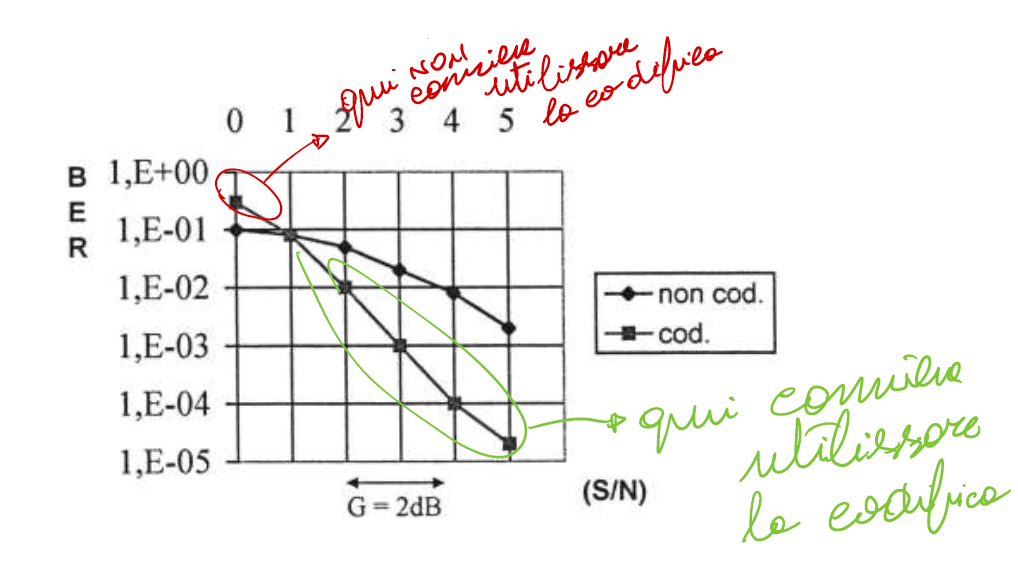
\includegraphics[scale = 0.8]{BER VS SNR.PNG}
\end{figure}

La scelta del codice va ottimizzata per la specifica applicazione. \newline 

In pratica, fissata la probabilità di errore di interessa, occorre cerca un codice il cui punto di incrocio con la curva non codificata sia al di sopra della regione di interesse, 
e che quindi garantisca un guadagno di SNR. \newline 

\newpage 

\section{Codici BCH}
\footnote{Slide del prof | Codifica di canale | pag 8 - 9 \\
Appunti di Damiano | pag 8 - 9 \\ 
Slide | Codifica di canale | pag  8 - 9\\ 
Appunti | 2025-04-15 | pag 9
}

Accanto ai codici semplici menzionati, esiste una famiglia di blocchi chiamati BCH (Bose-Chaudhuri-Hocquenghem, cioè i nomi dei ricercatori che per primi li proposero). \newline 

Grazie a questi codici possiamo possiamo scegliere dalla tabella del codice i possibili valori di n, k e t, come in questa tabella: 

\begin{figure}[h]
    \centering
    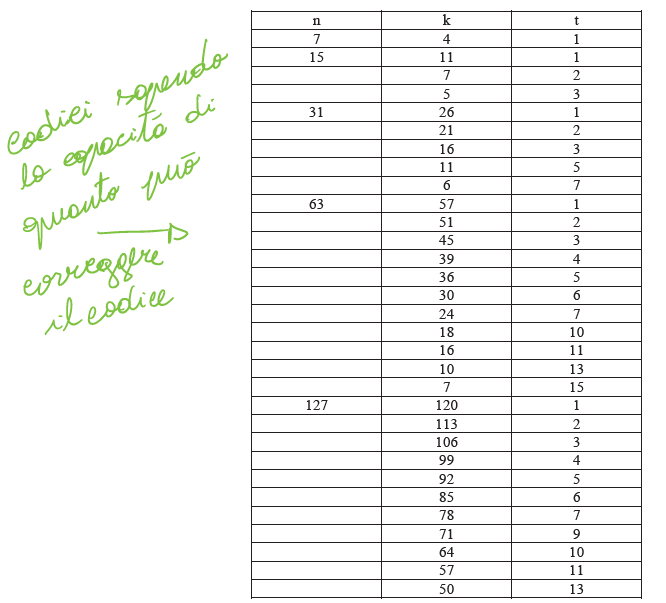
\includegraphics[scale = 1]{BCH Code esempio tabella.PNG}
\end{figure}

Se $p^{'}$ è sufficientemente piccolo, dell'ordine di $10^{-2}$ o meno, 
la $P_{Eb}$ diventa, considerando quella peggiorativa: 

{
    \Large 
    \begin{equation}
        P_{Eb}
        \approx
        \frac{1}{2}
        \cdot 
        \binom{n}{t+1}
        \cdot 
        p^{'^{t+1}}
    \end{equation}
}

Considerando invece quella approssimata non peggiorativa: 

{
    \Large 
    \begin{equation}
        P_{Eb}
        \approx
        \frac{2 \cdot t + 1}{n}
        \cdot 
        \binom{n}{t+1}
        \cdot 
        p^{'^{t+1}}
    \end{equation}
}

\newpage 

Utilizzando questa ultima formula, 
si può tracciare il grafico come il seguente: 

\begin{figure}[h]
    \centering
    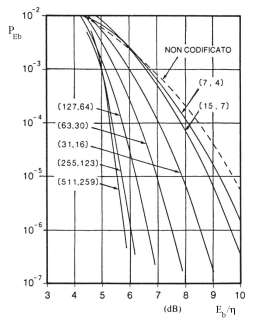
\includegraphics[scale = 2]{Curve BCH.png}
\end{figure}

In particolare, questo grafico mostra l'andamento del BER di diversi codici BCH. \newline

\newpage 

\section{Codici MDS}
\footnote{Slide del prof | Codifica di canale | pag 9 \\
Appunti di Damiano | pag 9\\ 
Slide | Codifica di canale | pag  9\\ 
Appunti | 2025-04-15 | pag 9
}

Considerando i codici in cui abbiamo una base M-aria, 
possono essere utili i codici Reed-Solomon (in breve RS). \newline 

I codici RS operano su un alfabeto di simboli M: 

{
    \Large 
    \begin{equation}
        M = 2^{m}
    \end{equation}
}

in cui: 

{
    \Large 
    \begin{equation}
        m > 1
    \end{equation}
}

Il codice RS fa parte della famiglia dei codici MDS (Maximum Distance Separable). \newline 

I codici RS vengono impiegati nella PPM per la registrazione ottica dei CD. \newline 

\newpage 

